\section{Case Studies}
\label{sec:cases}

\subsection{S\=amavedic notation: gating the withholding, not only the release}
\label{sec:case-samaveda}

The S\=amaveda is the Veda of chant, and its \=Arcika verses are printed in some
witnesses with svara marks indicating the melodic treatment of each syllable. This
layer is the project's sharpest test of the evidence model, for three reasons: the
marks are genuinely source-explicit, decoding them into pitch would be genuinely
interpretive, and the coverage is genuinely partial.

\paragraph{What was admitted.} 1{,}136 of the 1{,}844 \=Arcika verses carry an
accented witness (\cref{tab:samaveda}, \cref{fig:samaveda}), imported as a second
\code{TextVersion} of
the verse's own text in the role \code{PARALLEL\_TEXT}, never replacing the primary
text. We verified all of this against the live store: 1{,}136 accented parallel text
versions against 1{,}844 primary ones, and 25{,}542 tone marks on the accented rows.
Coverage is published as four figures rather than one --- \textsc{chanda} 471/585,
\textsc{aranya} 31/55, \textsc{mahanamnya} 3/10, \textsc{uttara} 631/1194 --- because
a single total of 1{,}136 hides which part of the \=Arcika a reader can and cannot
see notation for.

\paragraph{What was refused, and how the refusal is enforced.} The marks are recorded
as data and never decoded. The Kauthuma decipherment authority is not held, and a
study of a different school's chant was deliberately not applied. The refusal is
enforced at four levels rather than stated once: the row schema pins the payload to a
closed set of thirteen field names and checks that none of them names a pitch; the
predicate is the ordinary \code{HAS\_TEXT\_VERSION}, and a melodic predicate is
verified absent from the store's type table; the migration plan declares six explicit
refusals; and a live test scans every property key on the witness for pitch
vocabulary, permitting exactly one match --- the property that \emph{records} the
refusal. We confirmed the outcome: no melodic relationship type exists in the graph,
and the property \code{notation\_is\_interpreted\_into\_pitch} is present on all
1{,}136 witnesses with the value \emph{false}. A first version of that scan flagged
the guard as the thing it guards against, which is a small but exact illustration of
how hard it is to write a check that means what it says.

\begin{figure}[tbp]
\centering
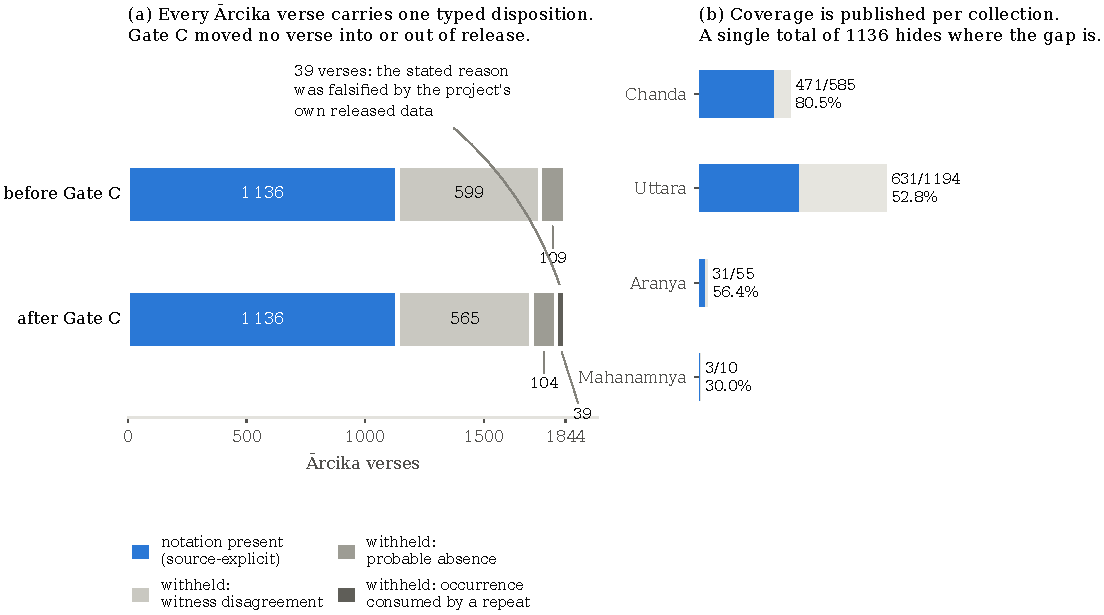
\includegraphics[width=\linewidth]{figures/fig_samaveda.pdf}
\caption{The S\=amavedic notation layer before and after the adversarial gate.
\textbf{(a)} Every one of the 1{,}844 \=Arcika verses carries exactly one typed
disposition. Gate~C moved no verse into or out of release; it added a third
withheld class and moved 39 verses into it, because the reasons those rows stated
were falsified by the project's own released data. \textbf{(b)} Coverage is
published per collection rather than as one total, because a total of 1{,}136 hides
which part of the \=Arcika a reader can and cannot see notation for.}
\label{fig:samaveda}
\end{figure}

% generated by figures-src/make_tables.py -- do not edit
\begin{table}[tb]
\centering
\caption{S\=amavedic notation: every one of the 1{,}844 \=Arcika verses carries
exactly one typed disposition, so a reader can never mistake a withheld verse for a
verse the tradition does not notate. The third withheld class did not exist until an
adversarial gate falsified the stated reasons of 39 rows.}
\label{tab:samaveda}
\small
\begin{tabularx}{\linewidth}{@{}lr>{\raggedright\arraybackslash}X@{}}
\toprule
Disposition & Verses & \\
\midrule
notation present, source-explicit & 1{,}136 & \footnotesize the witness prints marks on this verse \\
\quad withheld: near line, witness disagreement & 565 & \footnotesize needs philological adjudication \\
\quad withheld: no near line, probable absence & 104 & \footnotesize the witness may not carry the verse \\
\quad withheld: occurrence consumed by a repeat & 39 & \footnotesize \textbf{added by Gate C} (\cref{sec:case-samaveda}) \\
\midrule
\textbf{Total} & \textbf{1{,}844}
& \footnotesize verses with no disposition at all: \textbf{0} \\
\bottomrule
\end{tabularx}
\end{table}


\paragraph{Gate C, and the negative control.} The layer was audited by a gate
implemented separately from the pipeline that produced it, and the separation is
explicit: Gate C names the fields it refuses to read --- including the pipeline's own
tone-stripped text and its quality report --- and re-implements the declared
normalisation from the manifest's prose, using Unicode character categories rather
than the artefact's integer ranges. Eight attacks ran at full coverage over 6{,}232
row-evaluations.

The design feature we want to draw out is the second attack. Having re-derived each
verse's canonical text and found it aligned on 1{,}136 of 1{,}136, the gate then ran
the \emph{same} fold against the \emph{next} verse, and got 0 of 1{,}136. The gate's
own statement is the methodological point: the aligned result is only evidence to the
extent that this one is near zero. An agreement measurement without a negative
control does not distinguish a working method from a trivially satisfiable one.

\paragraph{The finding: 39 withheld rows whose reason the repository disproved.} Seven
attacks survived. The seventh did not, and it is the one that attacked the project's
own withholdings. 708 verses were withheld under two declared reason classes: 599
saying a near line exists so the difference needs philological adjudication, and 109
saying the accented witness plausibly does not carry the verse at all. The attack
observed that both claims are falsifiable from the repository itself --- if a
withheld verse's exact normalised text is \emph{released}, with notation, on a
coreferent twin elsewhere in the \=Arcika, then the witness demonstrably carries the
text and neither stated reason is the true mechanism.

Thirty-nine verses failed this test: 34 from the witness-disagreement class and 5
from the probable-absence class, each with at least one released twin carrying
byte-identical normalised text. The true mechanism was then measured rather than
guessed: of 202 repeated-text groups, 153 have every member released, so the witness
does print a repeated verse more than once and the harvest does find both lines.
Where only one member is released, the single order-consistent occurrence was
consumed by the earlier verse and the later one had no line left. That is line
exhaustion on a coreferent repeat --- neither an absence from the witness nor a
philological disagreement.

\paragraph{What changed, and what deliberately did not.} A third withheld class was
declared, \code{WITNESS\_OCCURRENCE\_CONSUMED\_BY\_A\_COREFERENT\_REPEAT}, and the
39 rows were moved into it; we read the corrected distribution off the live graph as
565 / 104 / 39, summing to the unchanged 708. \emph{No verse moved from withheld to
released, and no notation value was invented.} The gate's reasoning is that the
notated string belongs to the coordinate the witness printed it at, so copying a
twin's marks onto another verse would be inventing notation --- only the stated
reason changes. The original reason text is preserved verbatim on each corrected
row, and because the staging directory is a checksum-sealed artefact whose generator
is not in the repository, the correction was applied as an overlay rather than an
edit, leaving all twelve manifest checksums valid.

Finally, the failing run is preserved on disk and a test asserts that it still
records 39 defects, so the finding cannot be erased by regenerating only the passing
run. Gate C also declined to count the artefact's own pre-existing adversarial
sample, on the ground that it targets a different population and was run by the same
pass that produced it.

\paragraph{Why the gate existed at all.} An owner decision had released the notation
layer from an unrelated audio gate on four conditions, three of which measured met.
The fourth required that ``existing validation gates pass'' --- and the eligibility
record showed one gate \code{UNKNOWN} and the other \code{NOT\_RUN}. The condition
was recorded as unmet, with the reasoning that reading ``gates'' as the single gate
that already existed would clear the board by narrowing a word, and that the
conservative reading is the one that cannot manufacture a closure. A second owner
ruling confirmed the conservative reading, so the two gates were built rather than
the word narrowed. The newly built gate immediately landed a real defect.

\subsection{Translation: coverage is a kind, not a boolean}
\label{sec:translation}

Three separate mechanisms in this project once answered the question ``is this verse
translated?'' and all three answered it by testing for a translation edge. That test
was correct while every translation was a one-to-one rendering of its own verse, and
it stopped being correct the moment anything else was admitted.

\paragraph{Why alignment is hard here.} Five failure modes were measured, and none is
a data-quality problem that better sources would fix. The editions do not share a
verse spine: for a run of \emph{dvipada vir\=aj} hymns the canonical verses are single
hemistichs while the translator numbers the four-p\=ada group as one unit, printing
five units against ten verses. The available translation may be of a \emph{different
recension}: the standard English S\=amaveda is R\=a\d{n}\=ayan\=\i ya on its own
translator's preface, while this corpus is Kauthuma, and nine avenues were searched
without finding a public Kauthuma \=Arcika translation. Position cannot substitute,
because the offset between the two orders drifts monotonically from 0 to $-81$. The
source's own printed labels are sometimes wrong --- one book prints the sequence
23, 24, 23, 26, a misprint for 25. The corpus repeats itself, so ``same English,
different verse'' is normal rather than a defect; two of the packet's own duplication
tests were wrong for exactly that reason before the third was right. And a
translation can be present, correctly typed, and still invisible to a reader's edge
test, which is how a range alignment went unseen.

\paragraph{The typed model.} The replacement is two closed vocabularies and one
refusal. A \emph{coverage kind} says what a translation gives a verse --- dedicated,
range, container, or reused --- and is explicitly not rankable; the classifier
\emph{raises} on an unrecognised alignment level rather than defaulting, because
defaulting is how a fourth kind would silently be reported as a verse's own
translation. A \emph{verse coverage state} says what a verse has, in eight values of
which three are negative and distinguish genuinely different situations
(\cref{tab:coverage}). Alignment confidence is a six-valued typed vocabulary rather
than a number pretending to be a probability; the largest class, covering 17{,}095 of
18{,}427 renderings, is \code{MACHINE\_ALIGNED\_NO\_PER\_ROW\_CONTROL}, which names
its own weakness.

% generated by figures-src/make_tables.py -- do not edit
\begin{table}[tb]
\centering
\caption{Translation coverage as a typed state rather than a boolean. Each of the 20{,}210 mantras carries exactly one terminal state, so an absence always arrives with its reason attached. The two \code{UNCOVERED} states are distinct on purpose: one says a translated identical parallel exists elsewhere in the corpus, the other says nothing reaches the verse at all. The S\=amavedic column is the reason the distinction was built.}
\label{tab:coverage}
\small
\begin{tabular}{@{}lrrrrr@{}}
\toprule
Verse coverage state & RV & AV & YV & SV & Total \\
\midrule
\code{DEDICATED\_TRANSLATION} & 10{,}322 & 5{,}715 & 1{,}950 & 0 & 17{,}987 \\
 & \multicolumn{5}{@{}l@{}}{\footnotesize its own 1:1 English rendering} \\[2pt]
\code{RANGE\_TRANSLATION\_ANCHOR} & 30 & 34 & 0 & 0 & 64 \\
 & \multicolumn{5}{@{}l@{}}{\footnotesize anchors a print unit spanning it and others} \\[2pt]
\code{RANGE\_COVERED} & 36 & 52 & 0 & 0 & 88 \\
 & \multicolumn{5}{@{}l@{}}{\footnotesize carries no edge; named in another verse's span} \\[2pt]
\code{CONTAINER\_TRANSLATION} & 158 & 0 & 0 & 0 & 158 \\
 & \multicolumn{5}{@{}l@{}}{\footnotesize only rendering is aligned to a hymn} \\[2pt]
\code{REUSED\_RENDERING} & 0 & 21 & 0 & 173 & 194 \\
 & \multicolumn{5}{@{}l@{}}{\footnotesize another corpus's rendering of identical Sanskrit} \\[2pt]
\code{UNCOVERED\_REUSABLE\_PARALLEL\_AVAILABLE} & 0 & 6 & 0 & 1{,}488 & 1{,}494 \\
 & \multicolumn{5}{@{}l@{}}{\footnotesize nothing reaches it, but a translated identical parallel exists} \\[2pt]
\code{UNCOVERED\_NO\_RENDERING\_REACHES\_IT} & 6 & 11 & 25 & 183 & 225 \\
 & \multicolumn{5}{@{}l@{}}{\footnotesize nothing reaches it, and no parallel does} \\[2pt]
\midrule
\textbf{Total} & \textbf{10{,}552} & \textbf{5{,}839} & \textbf{1{,}975} & \textbf{1{,}844} & \textbf{20{,}210} \\
\bottomrule
\end{tabular}
\end{table}


\paragraph{What the S\=amavedic column shows.} 1{,}488 S\=amavedic verses are
uncovered \emph{but} have a translated identical parallel elsewhere in the corpus;
183 are uncovered with no parallel at all; and 173 carry a reused \d{R}gvedic
rendering admitted only on Sanskrit verified character-identical. The last of these
is the case the model was built for. Those 173 are visible to a reader, and they are
counted in no S\=amavedic translation figure: the code holds two frozen sets, one for
``English reaches the reader'' and one for ``independent English exists'', differing
by exactly the reused class, and records that a total reporting 173 English
translations for the S\=amaveda is wrong --- a mistake an earlier draft of the
staging made before the reuse column was checked. The independent-English count for
the S\=amaveda is zero.

\paragraph{Two disciplines worth naming.} First, the product shipped \emph{before}
the data: the import plan was built and hashed but deliberately not executed in the
commit that introduced the typed model, on the reasoning that the interface must be
able to represent a range and a reused rendering before such rows land, not
afterwards. Second, the campaign restated one of its own headline figures
\emph{downward} on purpose. Narrowing ``translated'' to mean a verse's own rendering
moved the \d{R}gvedic figure from 10{,}502 to 10{,}479, and a test now asserts the
range population beside it so that the narrowing cannot pass as a regression.

\paragraph{And a defect this found.} A prior import had attached 25 renderings to the
wrong verses, precisely because two editions did not share a verse spine and the
guard reported the mismatch as ``missing'' rather than as a spine divergence. The
rows were re-anchored and the readback was clean --- but the more useful artefact is
the reason code introduced alongside:
\code{SOURCE\_EDITION\_VERSE\_DIVISION\_DIFFERS}, which is now one of six typed
rejection reasons rather than an unexplained absence.
